\documentclass[lang=cn]{elegantpaper}

\title{十月份过程性研究记录}
\author{陶理}

\usepackage{amsmath}
\usepackage{tikz}
\usepackage{physics}
\usepackage[outline]{contour} % glow around text
\usepackage{xcolor}
\usepackage{graphicx}
\usetikzlibrary{intersections}
\usetikzlibrary{decorations.markings}
\usetikzlibrary{angles,quotes} % for pic
\usetikzlibrary{calc}
\usetikzlibrary{3d}
\contourlength{1.3pt}

\tikzset{>=latex} % for LaTeX arrow head
\colorlet{myred}{red!85!black}
\colorlet{myblue}{blue!80!black}
\colorlet{mycyan}{cyan!80!black}
\colorlet{mygreen}{green!70!black}
\colorlet{myorange}{orange!90!black!80}
\colorlet{mypurple}{red!50!blue!90!black!80}
\colorlet{mydarkred}{myred!80!black}
\colorlet{mydarkblue}{myblue!80!black}
\tikzstyle{xline}=[myblue,thick]
\def\tick#1#2{\draw[thick] (#1) ++ (#2:0.1) --++ (#2-180:0.2)}
\tikzstyle{myarr}=[myblue!50,-{Latex[length=3,width=2]}]
\def\N{90}

\begin{document}

\def\xmin{-0.7*\T}   % min x axis
\def\xmax{6.0}       % max x axis
\def\ymin{-1.04}     % min y axis
\def\ymax{1.3}       % max y axis
\def\A{0.67*\ymax}   % amplitude
\def\T{(0.35*\xmax)} % period
\def\f#1{\A*4/pi/(#1)*sin(360/\T*#1*Mod(\t,\T))} %Mod
\maketitle

\begin{abstract}
    该份过程性研究记录(截止至撰写日期)主要记录了十月上旬所完成的对于语音特征提取算法的学习以及对原理的剖析。截止至目前,我完成了对于傅里叶级数和傅里叶变换的理解,了解到了傅里叶变换在语音识别领域中的重要性,并对于傅里叶变换的计算有了初步的了解。
\end{abstract}
\section{傅里叶级数 \& 傅里叶变换}

目前许多音频特征提取算法是基于傅里叶变换的:如通过短时傅里叶变换 (STFT),将音频信号分成若干小段并将每一段进行傅里叶变换;通过梅尔频率倒谱系数 (MFCCs),使用STFT将信号转化为频谱图,再对频谱图进行处理。因此对于傅里叶变换的充分理解是完成一个好的音频特征提取的基础。

\subsection{傅里叶级数}
对于一个周期信号 $f(t)$,有:
\begin{equation}
    f(t) = \frac{a_0}{2} +\sum_{n=1}^{\infty} [a_n \cos(n\omega t)+b_n\sin(n\omega t)]
\end{equation}

通俗来讲,傅里叶级数就是将一个周期函数$f(t)$表示为无数个余(正)弦函数的和。

e.g. 假设有$g(t)$为一个方波,将其表示成无数个正弦函数的叠加,即下图所呈现。
\begin{center}
    \begin{tikzpicture}
        \message{^^JSquare wave synthesis - time}
        \def\xmin{-0.65*\T}  % max x axis
        \def\T{(0.465*\xmax)} % period
    
    % SQUARE WAVE
    \begin{scope}
        \clip ({-0.54*\T},-1.1*\A) rectangle (0.97*\xmax,1.1*\A);
        \foreach \i [evaluate={\x=\i*\T/2;}] in {-2,...,4}{
        \ifodd\i
            \draw[myblue!80!black!30,line cap=round] (\x,{-\A}) --++ ({\T/2},0);
            \draw[myblue!80!black!30,dashed,thin,line cap=round]
            ({\x+\T/2},{-\A}) --++ (0,2*\A);
        \else
            \draw[myblue!80!black!30,line cap=round] (\x,{\A}) --++ ({\T/2},0);
            \draw[myblue!80!black!30,dashed,thin,line cap=round]
            ({\x+\T/2},{\A}) --++ (0,-2*\A);
        \fi
        }
    \end{scope}
    
    % AXIS
    \draw[->,thick] (0,\ymin) -- (0,\ymax) node[left] {$y$};
    \draw[->,thick] ({\xmin},0) -- (\xmax,0) node[below=1,right=1] {$t$ [s]};
    
    % PLOT
    \draw[xline,samples=\N,smooth,variable=\t,domain=-0.55*\T:0.94*\xmax]
        plot(\t,{\f{1}});% node[pos=0.3,above] {$n=1$};
    \draw[xline,mygreen,samples=3*\N,smooth,variable=\t,domain=-0.54*\T:0.94*\xmax]
        plot(\t,{\f{1}+\f{3}});
    \draw[xline,myred,samples=5*\N,smooth,variable=\t,domain=-0.53*\T:0.94*\xmax]
        plot(\t,{\f{1}+\f{3}+\f{5}});
    \draw[xline,myorange,line width=0.7,samples=7*\N,smooth,variable=\t,domain=-0.52*\T:0.94*\xmax]
        plot(\t,{\f{1}+\f{3}+\f{5}+\f{7}});
    %\draw[xline,mypurple,samples=9*\N,smooth,variable=\t,domain=-0.52*\T:0.95*\xmax]
    %  plot(\t,{\f{1}+\f{3}+\f{5}+\f{7}+\f{9}});
    %\node[xcol,above=2,right=4] at ({720/\om},\A) {$x(t)=A\cos(\omega t)$};
    
    % NUMBERS
    \node[myblue,  above,scale=0.9] at ({0.16*\T},1.20*\A) {$s_1$};
    \node[mygreen, below,scale=0.9] at ({0.25*\T},0.88*\A) {$s_3$};
    \node[myred,   above,scale=0.9] at ({0.41*\T},1.17*\A) {$s_5$};
    \node[myorange,right,scale=0.9] at ({0.48*\T},0.50*\A) {$s_7$};
    
    % TICKS
    \tick{{  \T},0}{90} node[below right=-2,scale=0.8] {$T$};
    \tick{{2*\T},0}{90} node[below right=-2,scale=0.8] {$2T$};
    %\tick{{2*\T  },0}{90} node[right=1,below=-1,scale=0.8] {\contour{white}{$2T$}};
    \tick{0,{ \A}}{  0} node[left=-1,scale=0.9] {$A$};
    \tick{0,{-\A}}{180} node[right=-2,scale=0.9] {$-A$};
    
    \end{tikzpicture}
\end{center}

其中,$g(t)$就可以表达为:
\begin{equation}
    g(t)=\frac{4A_{\max}}{\pi}\sum_{n=1}^{\infty}\frac{\sin((2n-1)\omega t)}{2n-1}
\end{equation}
\subsection{傅里叶变换}
\begin{equation}
    F(\omega)=\int f(t)\cdot e^{(-i\omega t)}\cdot dt
\end{equation}

简单来讲,傅里叶变换是傅里叶级数的拓展,可以将非周期函数转化为多个余(正)弦函数的和。实际上,可以将傅里叶级数是傅里叶变换在周期函数上的特例。

傅里叶变换的意义:为研究信号的频谱特性提供了方案,提供了一种将时域信号转化为频域信号的方法。

傅里叶变换在语音识别领域的意义:傅里叶变换使得时域上的音频信号转化为频域上的信号,从而对于研究音频的特征提供了方案。
\begin{figure}
    \centering
    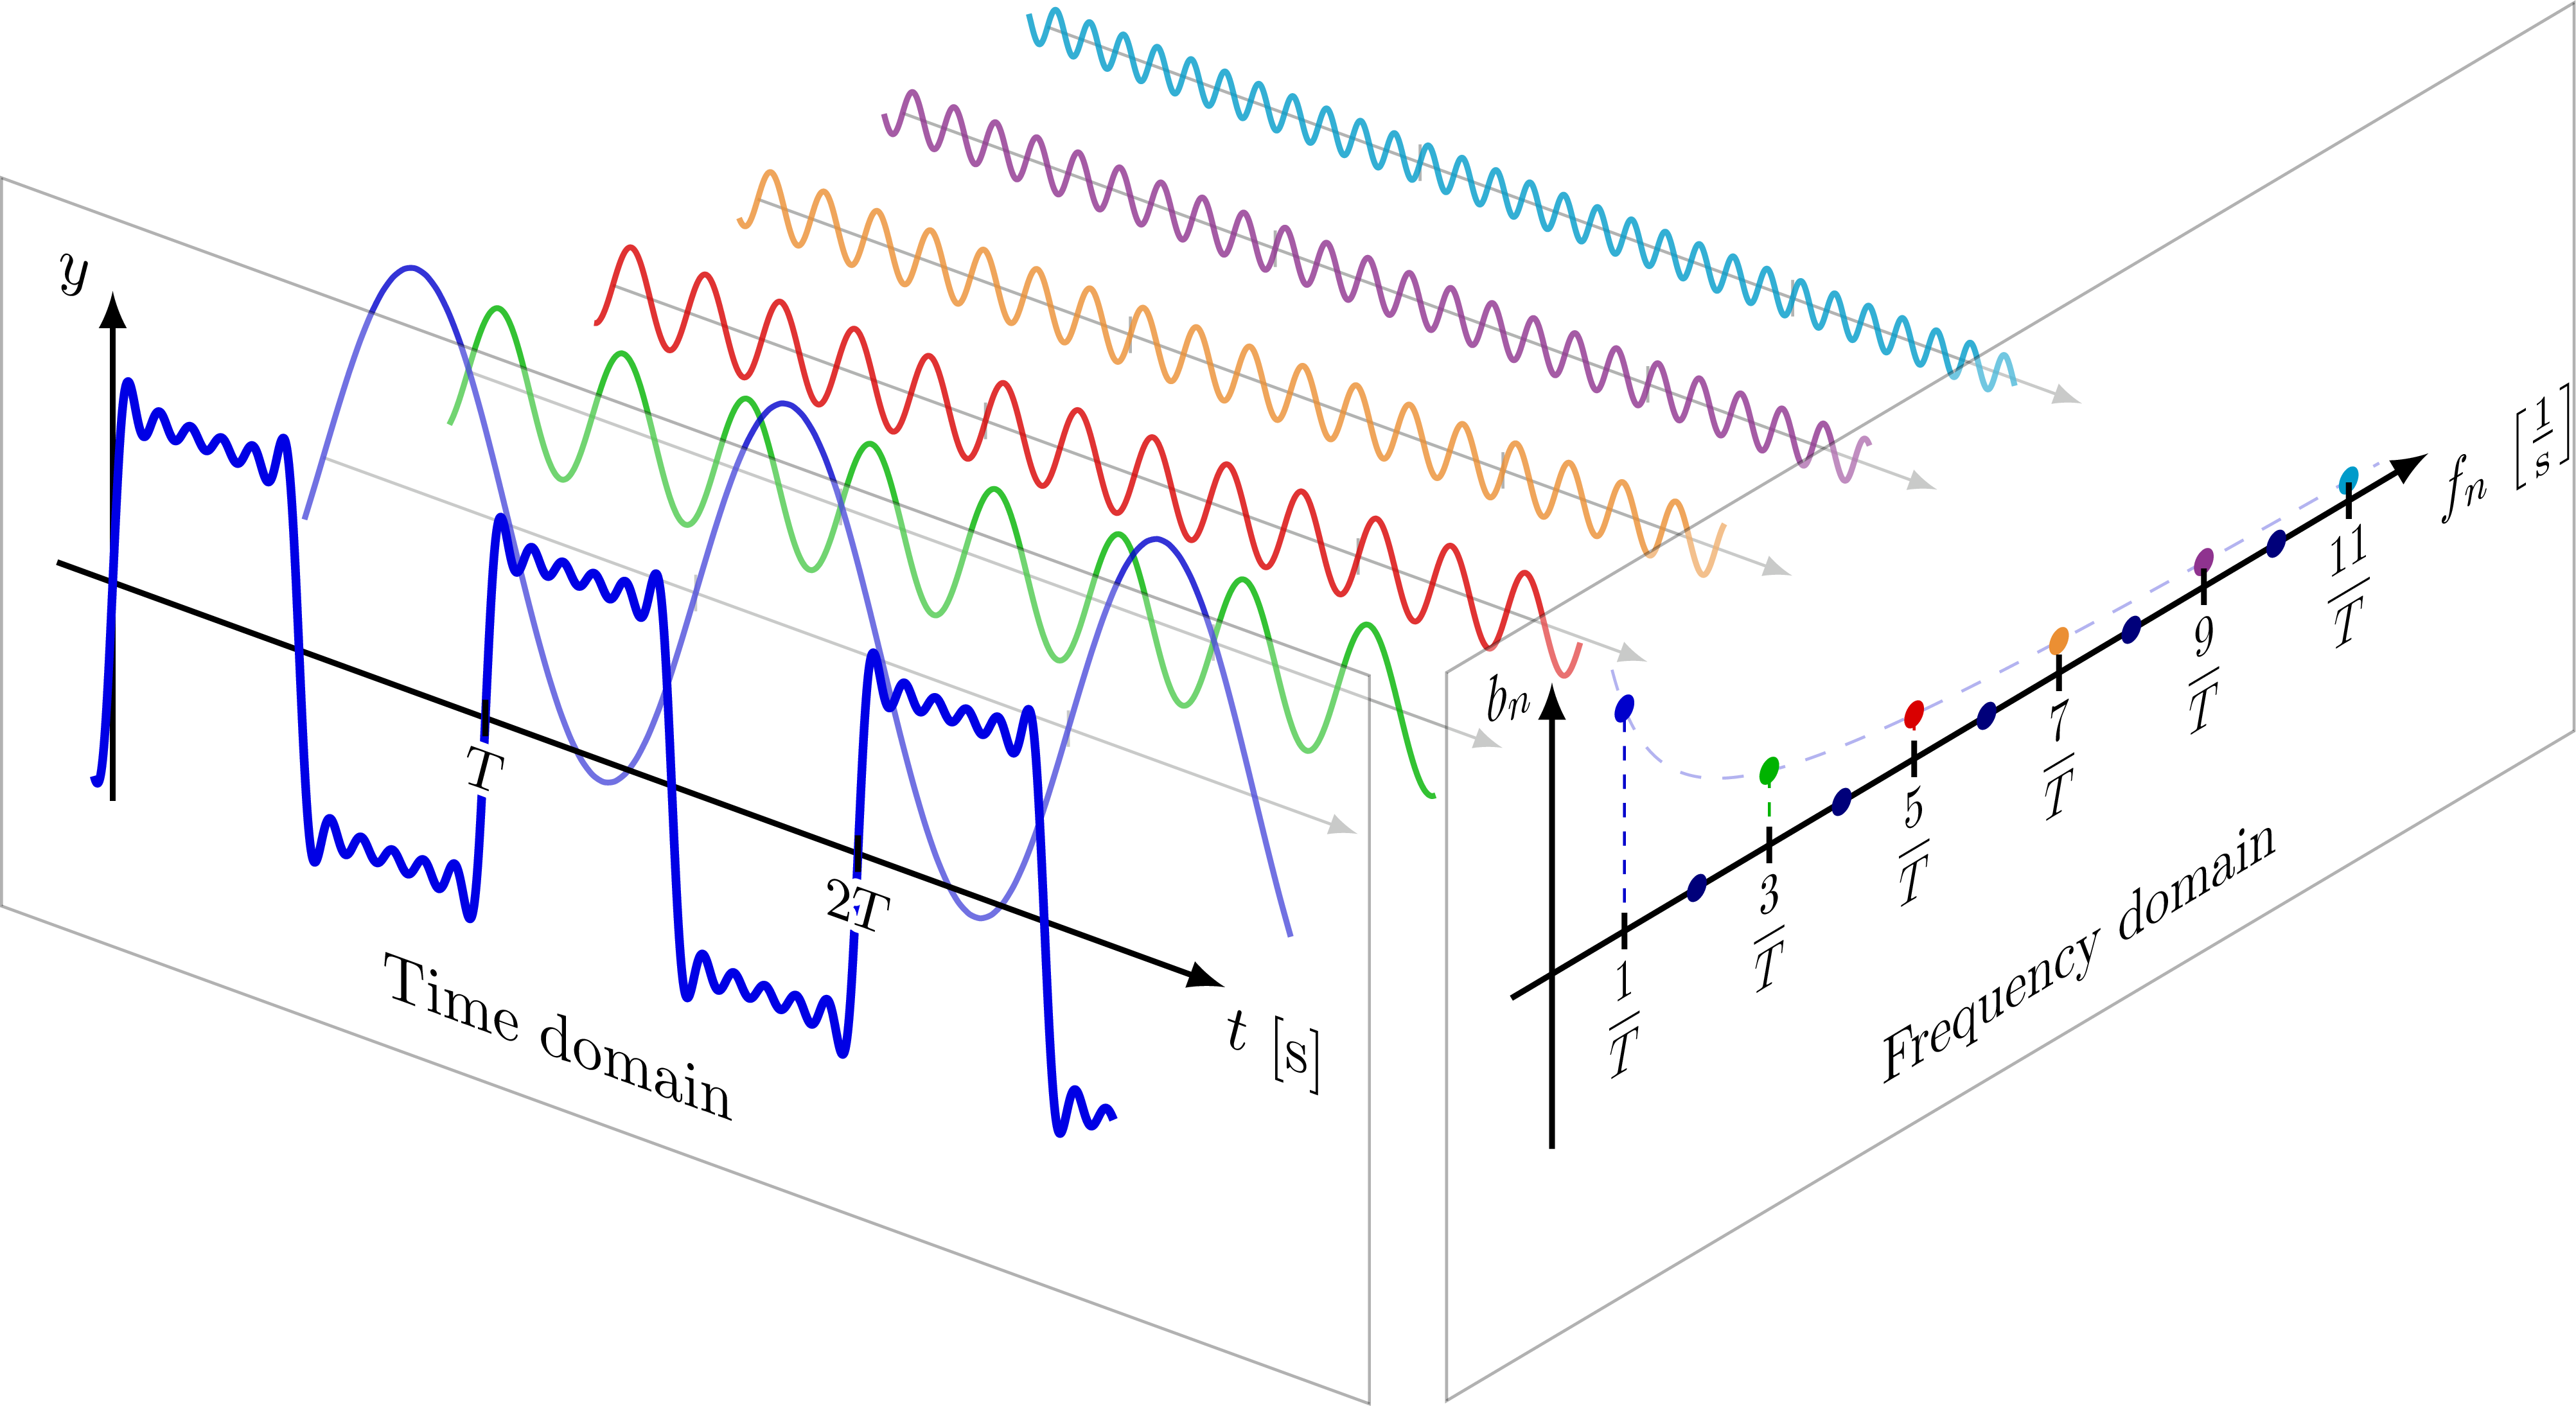
\includegraphics[scale=0.05]{Fourier Transform.png}
\end{figure}
\section{语音特征提取算法}
\subsection{短时傅里叶变换}
短时傅里叶变换,即Short Time Fourier Transform,简称STFT。

由于傅里叶变换将时域信号转化为频域,所以无法从傅里叶变化后的信号观察出特定时刻的频率,所以通过“加窗”的手段,将音频分为多个小的片段,如此即能将每一个小片段看作平滑的曲线,再进行傅里叶变换,就可以知道在每个时刻上的频率。

\begin{figure}[h]
    \centering
    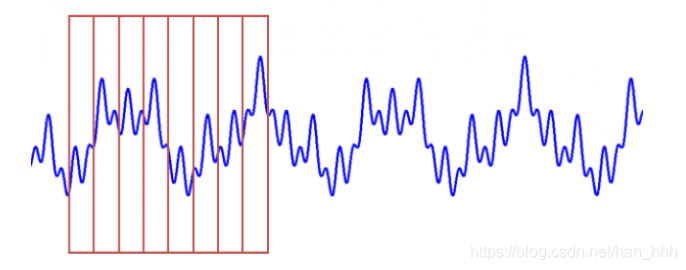
\includegraphics[scale=0.4]{STFT.png}
\end{figure}

\subsection{梅尔频率倒谱系数}
梅尔频率倒谱系数,即Mel-scale Frequency Cepstral Coefficients,简称MFCCs。梅氏系数也是在语音识别领域中运用的最为广泛的特征提取算法之一。
梅尔频率倒谱系数通常有以下几个步骤 以下引自百度百科 \textit(https://baike.baidu.com/梅尔频率倒谱系数/2916505) :

\begin{enumerate}
    \item 将一段语音信号分解为多个讯框
    \item 将语音信号预强化,通过一个高通滤波器。
    \item 进行傅立叶变换,将信号变换至频域。
    \item 将每个讯框获得的频谱通过梅尔滤波器(三角重叠窗口),得到梅尔刻度。
    \item 在每个梅尔刻度上提取对数能量。
    \item 对上面获得的结果进行离散傅里叶反变换,变换到倒频谱域。
    \item MFCC就是这个倒频谱图的幅度(amplitudes)。一般使用12个系数,与讯框能量叠加得13维的系数。
\end{enumerate}

以下为我通过Python语言编程所完成的程序结果:
\begin{figure}[h]
    \centering
    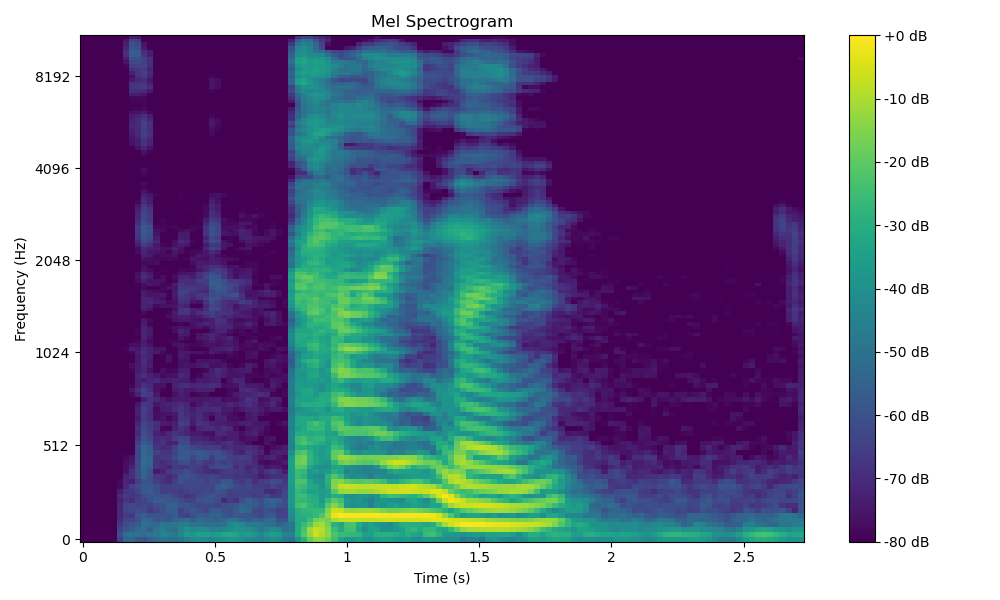
\includegraphics[scale=0.4]{MFCC.png}
\end{figure}
\end{document}
